\documentclass{article}
\usepackage[colorlinks]{hyperref}
\usepackage{pgfplots}
\usepackage{parskip}
\usepackage{subcaption}
\usepackage{minted}
\usepackage{mdframed}
\usepackage{color}
\usepackage{verbatim}
\usepackage[
  hmargin={1.3in,1.3in},
  vmargin={1in,1in},
  includefoot,
  footskip=30pt,
]{geometry}

\pgfplotsset{compat=1.13}

\pgfplotsset{every axis legend/.append style={legend pos=outer north east, font=\footnotesize}} 

\newcounter{codecounter}

\newcommand{\mycode}[4]{
  \vspace{1em}
  \begin{mdframed}[backgroundcolor=DarkGray, topline=false,bottomline=false,leftline=false,rightline=false]
  \refstepcounter{codecounter}Algorithm \thecodecounter: #2 \label{#1}
  \end{mdframed}
  \begin{mdframed}[backgroundcolor=LightGray, topline=false, bottomline=false, leftline=false, rightline=false]
    \inputminted
    [
      baselinestretch = 1.2,
      %fontsize        = \footnotesize,
      linenos,
      mathescape  = true,
      firstnumber = 1,
      fontsize=\small
    ]{#4}{#3}
  \end{mdframed}
  \begin{mdframed}[backgroundcolor=DarkGray, topline=false,bottomline=false,leftline=false,rightline=false]
  Algorithm \thecodecounter: #2
  \end{mdframed}
  \vspace{1em}
}

\usepackage{xcolor}
\definecolor{DarkGray}{gray}{0.7}
\definecolor{formalshade}{rgb}{0.95,0.95,1}
\definecolor{darkblue}{rgb}{0.21,0.24,59}
\definecolor{LightGray}{gray}{0.95}

\title{CS 267: Homework 3}
\author{Richard Barnes, Danny Broberg, Jiayuan Chen}
\date{April 5, 2016}

\hypersetup{
  pdfauthor={Richard Barnes, Danny Broberg, Jiayuan Chen},
  pdftitle={CS 267: Homework 3},
  pdfproducer={LaTeX},
  pdfcreator={pdfLaTeX}
}

\begin{document}
\maketitle

\section{Introduction}
This report describes our implementation of a de novo genome DNA assembly program using Unified Parallel C (UPC). UPC is an extension of the C language, outfitted for a Partitioned Global Address Space (PGAS) programming model. This model associates memory physically with specific processes but enables shared access. This bears syntatic similarities to OpenMP and other shared memory programming models.

Our paper is organized as follows:
\begin{enumerate} %TODO: Rewrite
\item description of the computational resources
\item a section that describes the general serial algorithm approach
\item a section that describes the general extension to UPC
\item evaluation of the code's performance
\end{enumerate}

\section{Machine Description}
For our codes we use NERSC's Edison machine. The machine has 5,576 compute nodes. Each node has 64GB DDR3 1866\,MHz RAM and two sockets, each of which is populated with a 12-core Intel ``Ivy Bridge" processor running at 2.4\,GHz. Each core has one or two user threads, a 256 bit vector unit, and is nominally capable of 19.2 Gflops. Notably, for our purposes, each core has its own L1 and L2 cache. The L1 cache has 64\,KB (32\,KB instruction cache, 32\,KB data) and the L2 cache has 256\,KB. The 12 cores collectively share a 30\,MB L3 cache. The caches have a bandwidth of 100, 40, and 23 Gbyte/s, respectively.\footnote{\url{http://www.nersc.gov/users/computational-systems/edison/configuration/}} Both the L1 and L2 caches are 8-way and have a 64 byte line size.\footnote{\url{http://www.7-cpu.com/cpu/IvyBridge.html}} 


\section{The Algorithm}
Sequencing long strands of DNA is difficult and time-consuming. For strands beyond a certain length it may not even be technically feasible. Therefore, faster and more scalable methods have been developed. Shotgun de novo genome assembly breaks a long piece of DNA into many shorter segments. These segments can be easily sequenced.

The problem then is to reassemble the original DNA by fitting the pieces together. In the simplified data set given here, the data takes the form of contiguous sequences of 19 or 51 bases (henceforth, a ``kmer") with known prefixes and suffixes. We are guaranteed that each kmer is unique. Together, the kmers a De Bruijn Graph.

Our program will construct this graph and traverse its connected components. To do this, a hash table will be used to store nodes of the graph with hashed kmers acting as keys. The values of the hash table will correspond to the prefix and suffixes and, thereby, serve as edges linking the nodes together.

Our algorithm begins by detecting how many kmers are in the input. It then allocates a shared memory hashtable three times larger than this number. Members of the hashtable are stored via open addressing with linear probing: this is wasteful of memory, but greatly simplifies the data structure, thereby reducing the potential for errors. Using a hashtable of size $3N$ ensures that occupancy stays well below 70\%, a point at which performance has been empirically shown to degrade significantly.

Kmers are hashed using Dan Bernstein's \texttt{djb2} hash function. Tests using the small data set with Austin Appleby's \texttt{MurmurHash3} didn't show a significant reduction in collisions. Since kmer elements are drawn from a library of four symbols, only 2-bits of information are required to represent each symbol. Therefore, as kmers are read they are transformed to this more compact representation.

Additionally, a local array of pointers to the hash table is allocated. As the process reads kmers and adds them to the hash table, it makes a note of which kmers have prefixes indicating that they begin sequences and uses this local array to store that information. These starting-kmers (smers) form the starting points of the graph traversals which generated the contiguous (output) sequences. One might worry that storing smers locally would result in them being unevenly distributed; however, this is not a problem if we assume (a)~that the smers are distributed evenly throughout the file and (b)~that the smers, on average, are part of components of approximately equal size. These assumptions are reasonable because it is possible to randomize the order of the lines in the input file, which means that smers are evenly distributed and, therefore, component sizes should therefore be as well. For the purposes of the assignment, we do not randomize the input, but do verify that the assumption is at least nominally fulfilled by the test data provided as shown in Figures~\ref{fig:smer_dist_small} and \ref{fig:smer_dist_large}.

\begin{minipage}{\linewidth}
  \captionsetup{type=figure}
  \begin{center}
  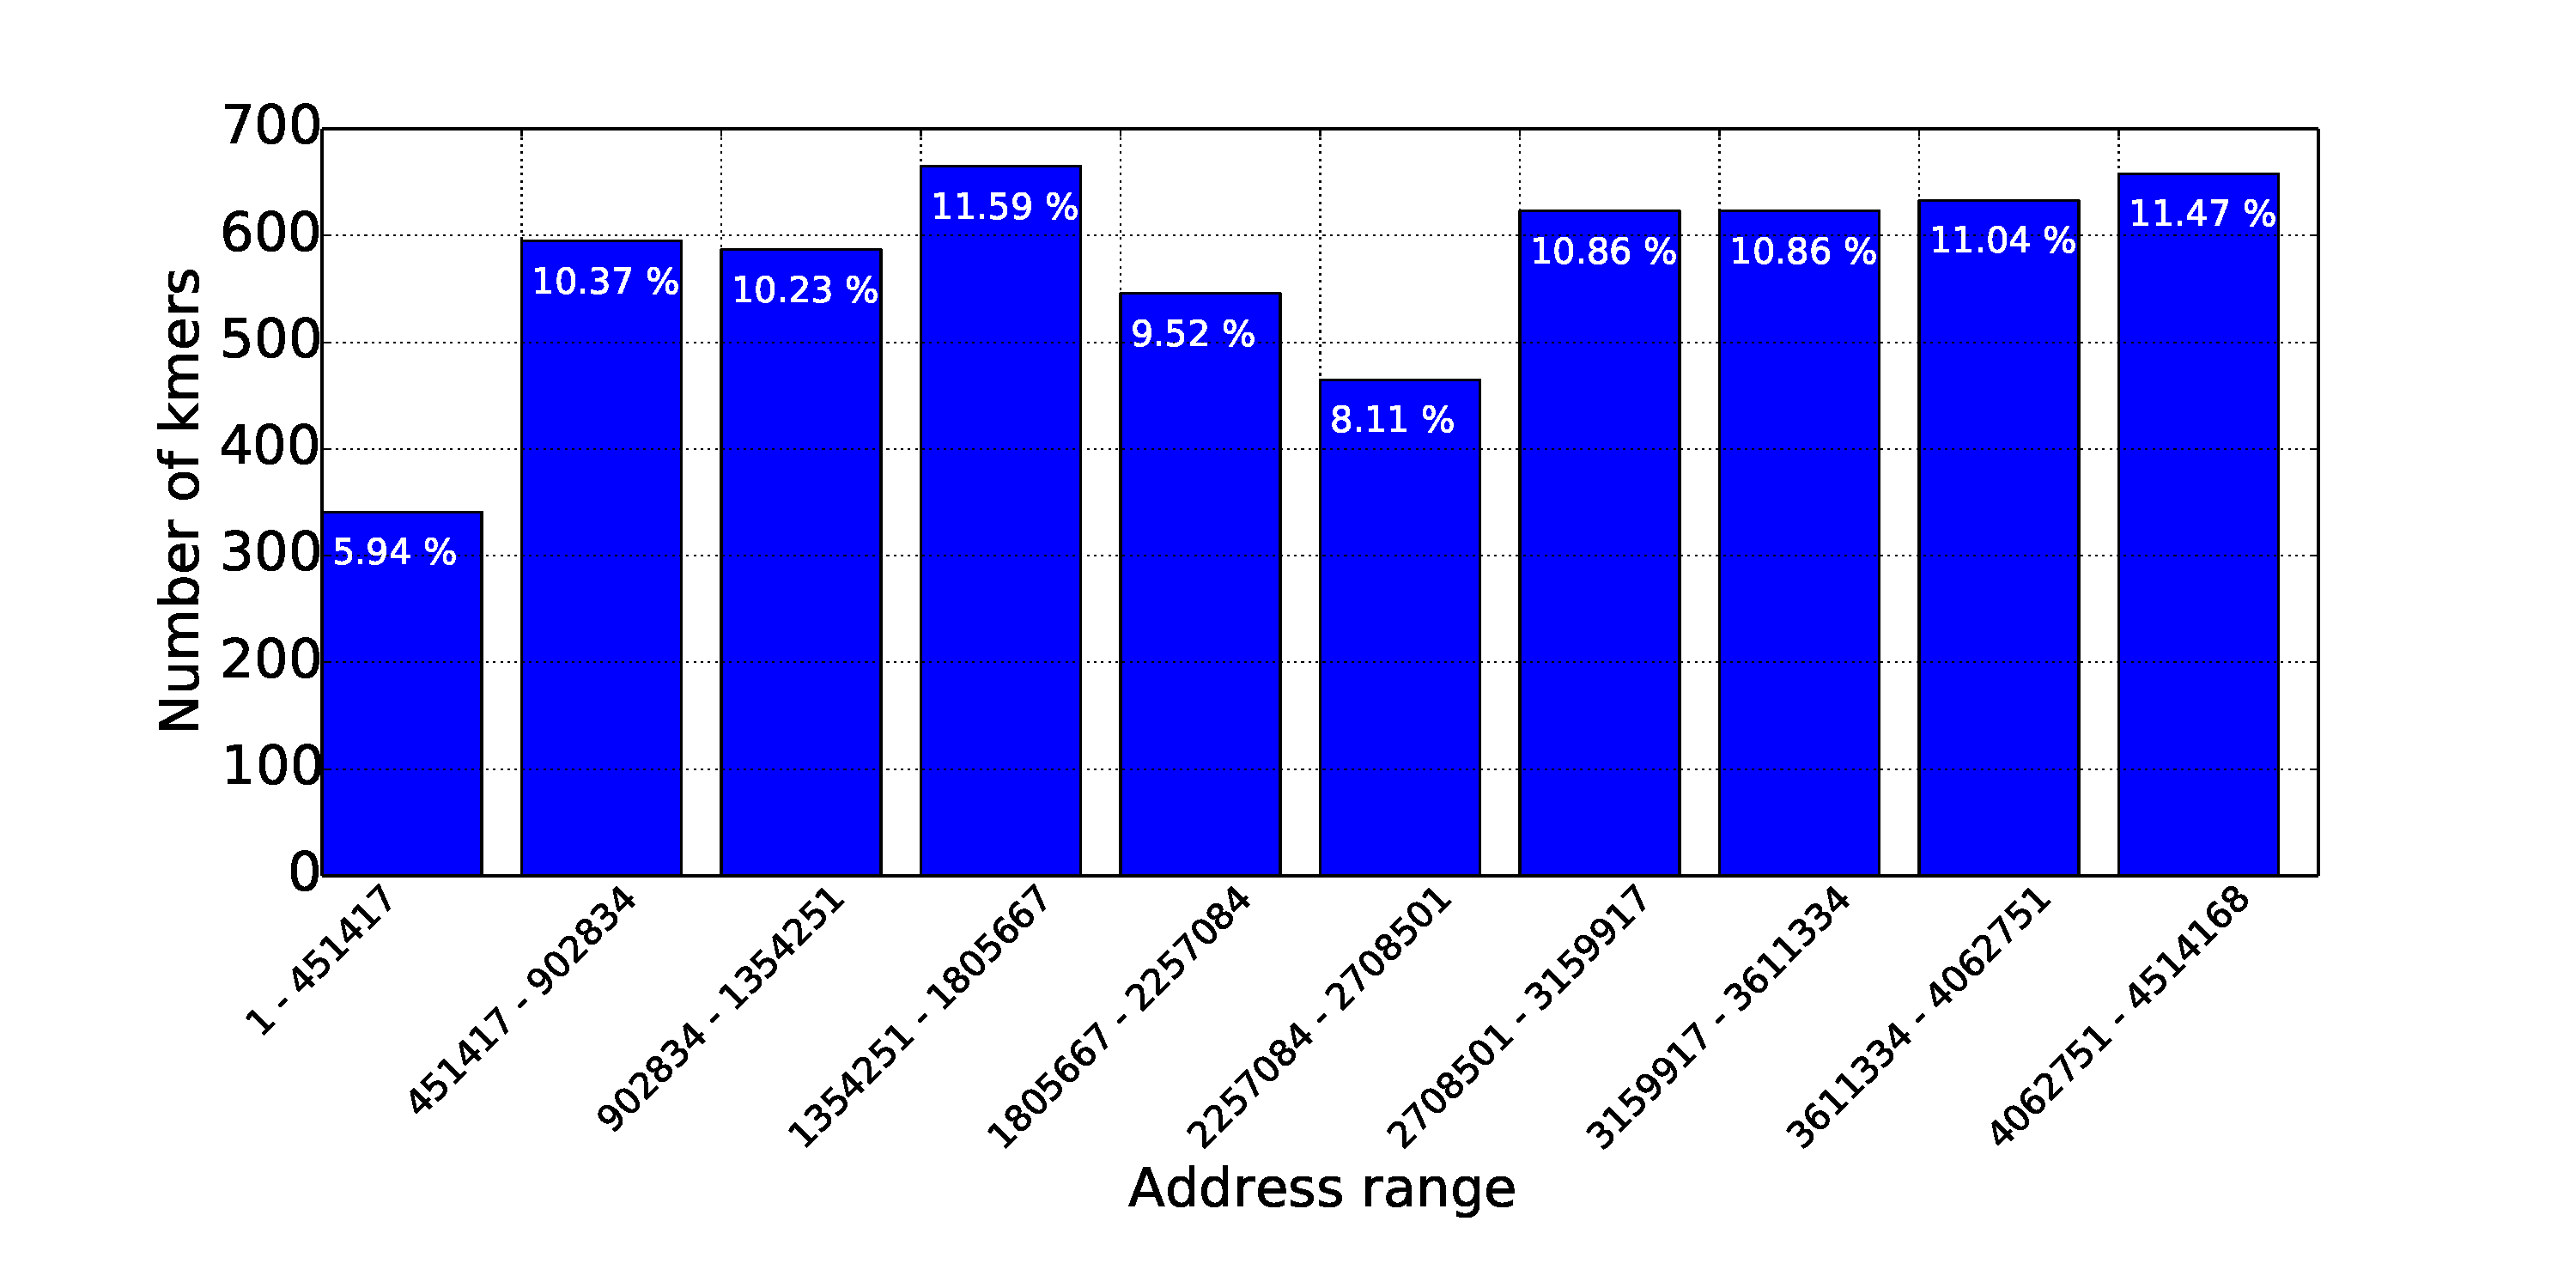
\includegraphics[width=0.8\textwidth]{shorthisto.pdf}
  \end{center}
  \caption{Distribution of start kmers to address space (Small data set)} \label{fig:smer_dist_small}
\end{minipage}

\begin{minipage}{\linewidth}
  \captionsetup{type=figure}
  \begin{center}
  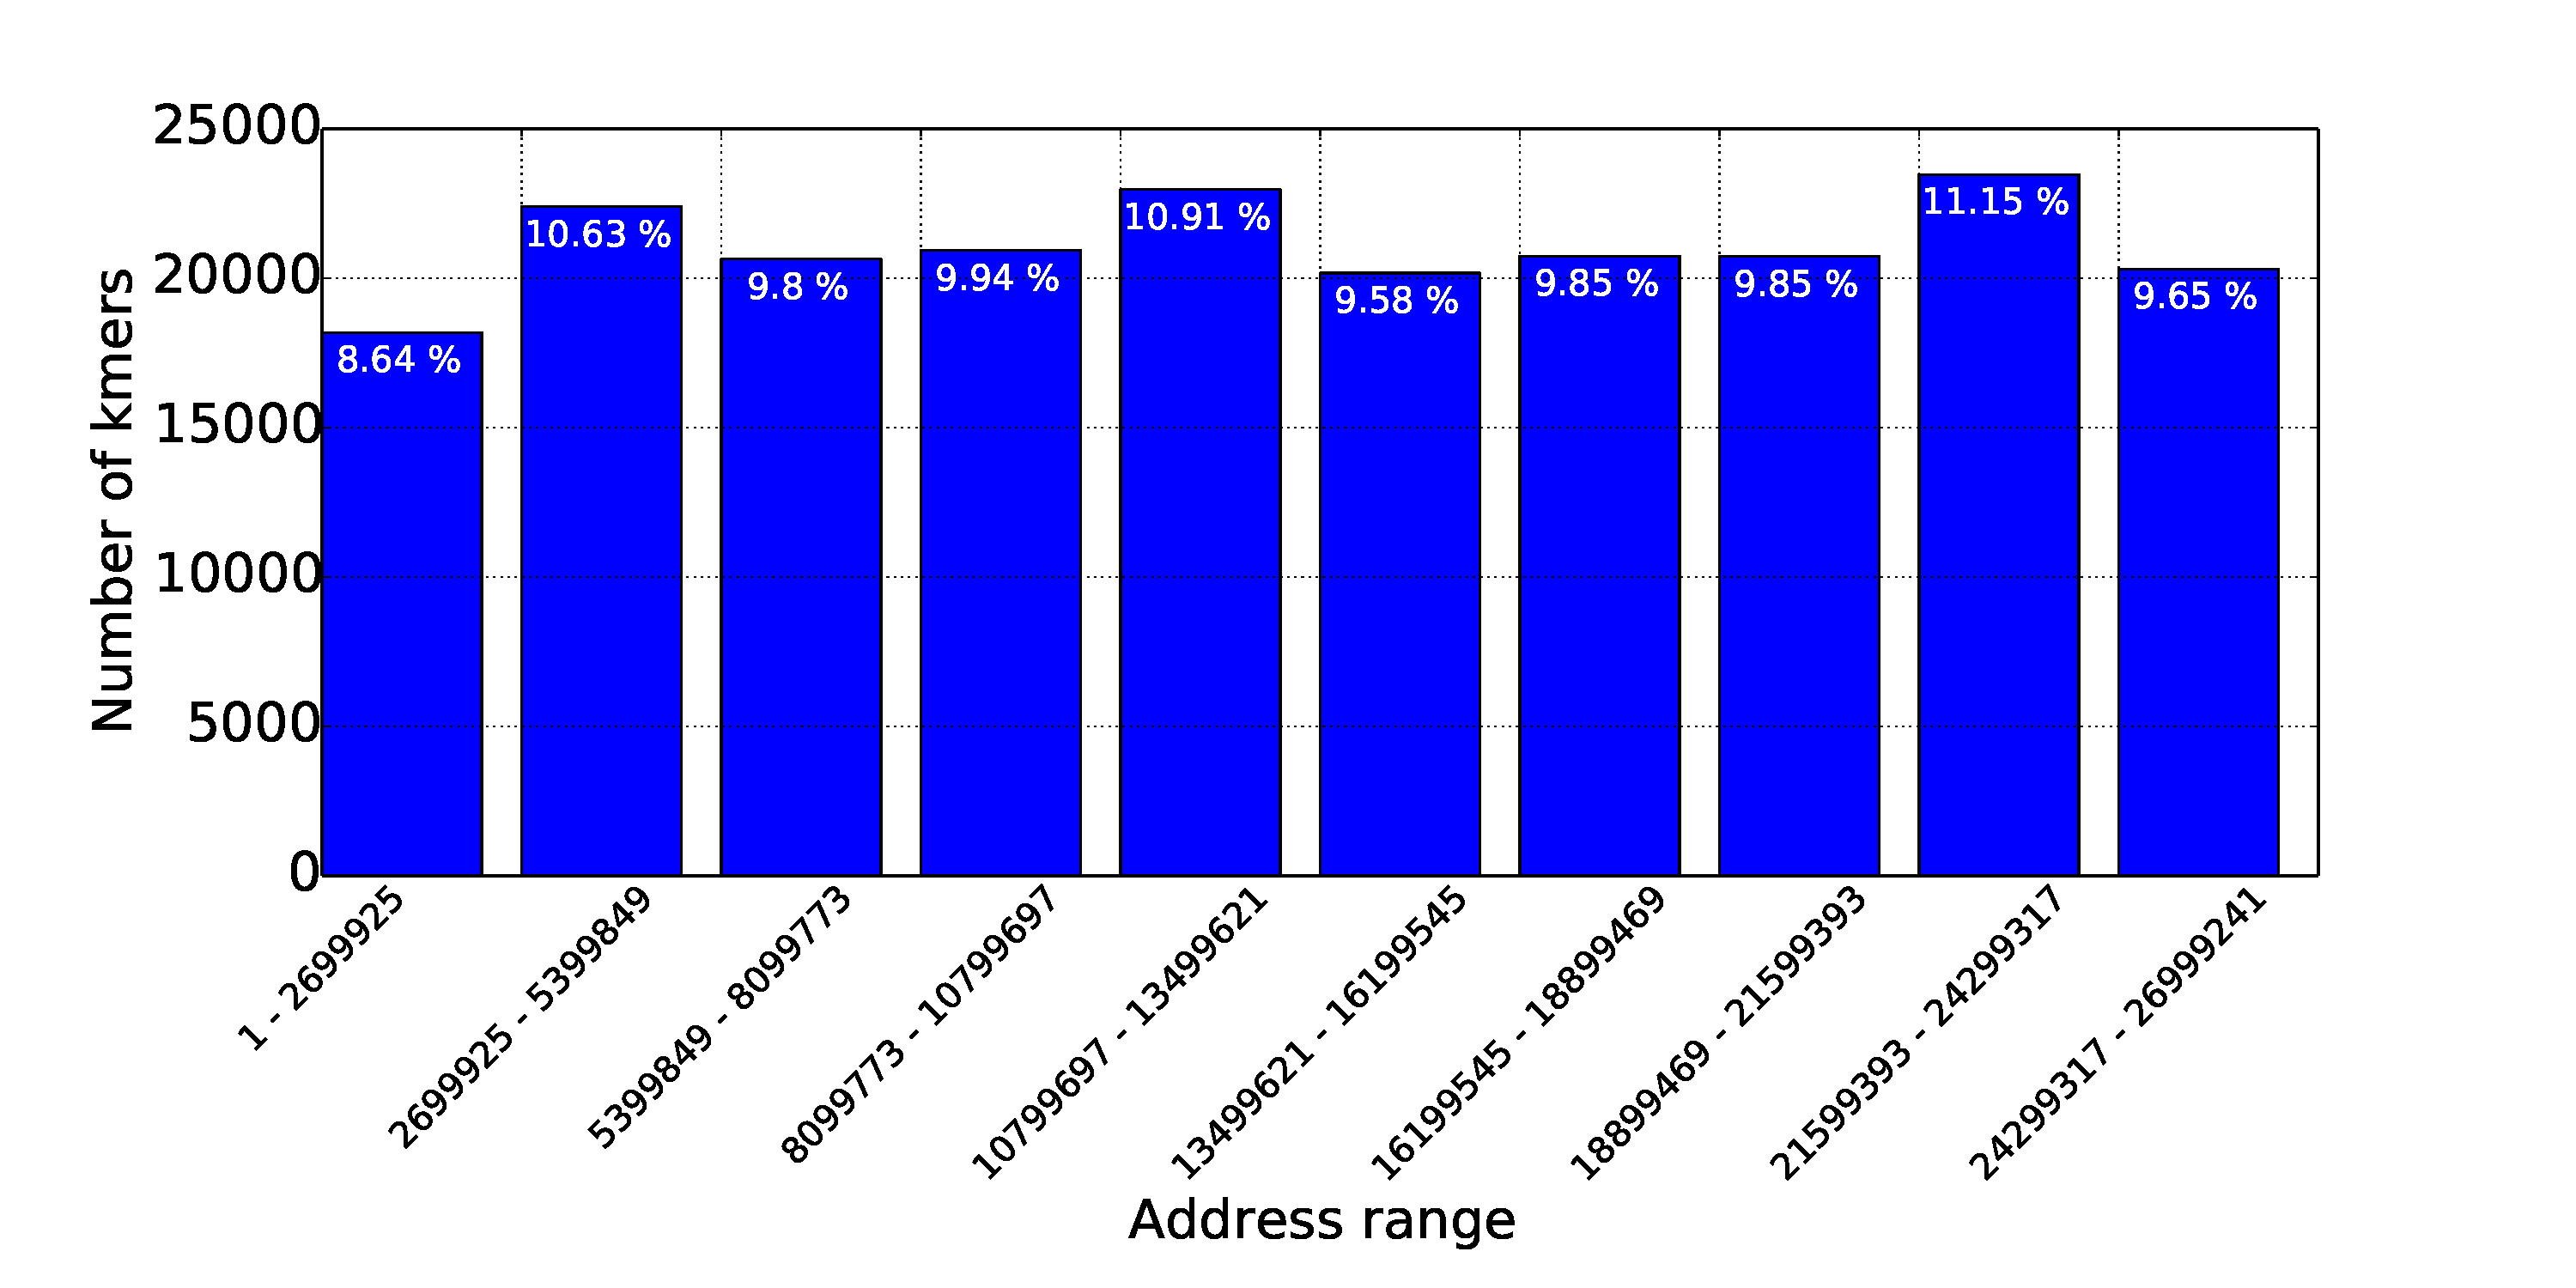
\includegraphics[width=0.8\textwidth]{longhisto.pdf}
  \end{center}
  \caption{Distribution of start kmers to address space (Long data set)} \label{fig:smer_dist_large}
\end{minipage}

Since the size of the file and the number of threads/processes can be determined at run-time, it is possible to assign threads to read separate, non-overlapping blocks of lines from the file. Each process begins reading and, as it does so, adding kmers. 

In our algorithm, adding a kmer is a two-step process. If a kmer hashes to an address owned by the process which read it, then the process saves the kmer to that address immediately. If, however, the kmer hashes to an address which is not owned by the process, then the process adds the kmer to a linked list in its private local storage: the kmer will be added to the shared space later. This scheme guarantees that kmers being added to the hashtable do not encounter race conditions.

After all of the kmers have been read in this way, the kmers stored in the linked lists must be added to the hashtable. But race conditions must be avoided. One way to do this is to lock addresses or, more practically, blocks of addresses. But locks can create performance bottlenecks and introduce the possibility of deadlocks.

Therefore, the hashtable is divided into evenly-sized and sequential blocks based on the number of threads. Each thread is given exclusive access to a block and deposits that block's associated kmers from its linked list. A barrier synchronizes the threads and then each thread does the same operation with the next block until each thread has seen every block.

This round robin distribution must be performed twice because kmers may hash to filled slots in the table and, in the course of linear probing, be slotted for insertion into an address outside the block the kmer's depositing thread currently has access to. However, twice is guaranteed to be sufficient because the 33\% maximum occupancy of the hash table coupled with the uniform distribution of the hash function guarantees that there will be sufficient slots in each block such that no kmer will move across more than one boundary via linear probing. UPC's default strict memory operation ordering guarantees that this round robin approach will not have race conditions since each thread has exclusive access to the memory it is manipulating and operations performed on that memory are guaranteed to be performed in sequential order.

As the kmers are inserted into the hashtable, they are removed from the linked list. It is therefore simple to check that all kmers have been added: the list will empty if this is the case. As the kmers are inserted into the hashtable, the smers are noted and their final addresses saved to their inserting thread's private local memory.

Once all of the kmers have been added to the hashtable, each thread iterates through its saved smers and traverses the table. No special synchronization is needed for this step because only read operations will take place.

Kmers are read from a striped file. Such a file is distributed into blocks across multiple hard drives, which can increase data throughput. We don't expect to see much benefit from this when running on a single node due to contention for that node's connection with memory; however, when running across several nodes there may be a large benefit.

For maximum benefit, each process should read memory from a separate part of the file, with no overlap. However, this is difficult to achieve if the number of processes might change. Therefore, the block size is chosen to be considerably smaller than the amount of data a process will read in. The effect is that the processes cycle between which drive they are getting data from. We do not attempt to synchronize this cycling and it is difficult to analyze theoretical (given potentially different read rates), but the ultimate effect is less contention than would be expected if everything were read from a single hard drive. For similar reasons, we write outputs to the scratch space for our tests.

\section{Design Choices and Optimizations}
We made three major design choices: (a)~using open hashing with linear probing rather than separate chaining, (b)~using round robin exclusive access rather than locks, (c)~strip and memory blocking decisions.

The choice to use open hashing with linear probing (a) was motivated by a desire for a simple algorithmic design which avoided complex structures in shared memory. For good performance, this design requires a hash function which not only provides a uniform distribution, but also even spacing to minimize collisions. We did not verify that \texttt{djb2} provides this, but reduced fallout from a bad hash spacing by using a $3N$-sized hashtable.

Separate chaining guarantees immediate insertion and retrieval proportional to bin occupancy whereas open hashing provides insertion and retrievals which are both proportional to the number of adjacent occupied addresses. Therefore, separate chaining is likely to have faster insertion times. Again, using a sufficiently large hashtable, as we have, reduces this problem.

Therefore, we expect the only downside to our choice of open hashing to be the wasted memory. However, given the sizes of the datasets here, this is not problematic for us.

The choice to use round robin kmer insertion (b) rather than locks was also motivated by design simplicity. Shared memory structures and deadlock potential were entirely avoided by this design. We therefore expect that this choice should be both faster and safer than alternative designs. An earlier alternative design we tried was to use atomic conditional-updates to write to relevant memory locations; however, these accesses were implemented as simple locks and not available on all of the UPC compiles we used. Thus, they added complexity with few additional benefits.

Testing the foregoing assertions would require significant redesign of our algorithm, which we did not have time to do. Therefore, we rely on our arguments above as justification of the choice.

Our choice of file striping patterns and UPC memory blocking (c) provides another potential avenue for optimization. However, long queue times on Edison interfered with carrying out systematic tests.

\section{What About MPI?}
UPC was perhaps the largest design choice we made. (Of course, it wasn't really a choice because part of the assignment was to use it.) Using a two-sided communication paradigm, like MPI would necessitate a few changes to our algorithm.

The simplest approach would be to have each thread allocate a portion of memory corresponding to part of the hashtable. As in our algorithm, each thread can then write to its portion of the hashtable and save kmers corresponding to other threads' address blocks in a list in its local memory. Since each thread knows which thread will ultimately own these saved kmers, the thread can send them directly to their owner using non-blocking I/O. Once they have all been sent, the thread can use blocking I/O to receive the additional kmers it owns from other threads. If this fills a message buffer, then the threads could alternate between send and receive modes several times if necessary.

Now each thread owns a part of the hashtable and a set of smers. Each thread will have approximately the same number of smers because the smers were evenly distributed in the input (see above). For each kmer, a thread sends a message to the node which owns that kmer's hash and receives back the value of the hash. Since each thread is doing this, threads must interleave work on their contigs with replies to incoming requests for values. Therefore, sends should be non-blocking and the thread should be able to receive messages whose tag corresponds to either to values being returned or values being requested.

Race conditions for data will not occur here because each thread always has exclusive access to its own memory. Separate chaining is useful in this instance because then thread which owns an address can always be accurate predicted (i.e.\ there is no need for value or hashtable-write requests to be forwarded on to another thread).

\section{Results}

Figure~\ref{fig:small_single_times} shows the absolute run-times of our algorithm on the small dataset for varying numbers of threads. We also processed the small dataset across eight nodes with a much larger number of processors. As Figure~\ref{fig:small_mult_times} shows, using about eight threads on a single node is faster than the fastest time achieved running on many threads across many nodes. For this small dataset, the processing power of each thread is probably under-utilized and communication overhead likely dominates the time-to-completion. Therefore, we only analyze the small dataset in terms of running on a single node.

\begin{minipage}{\linewidth}
  \captionsetup{type=figure}
  \begin{center}
  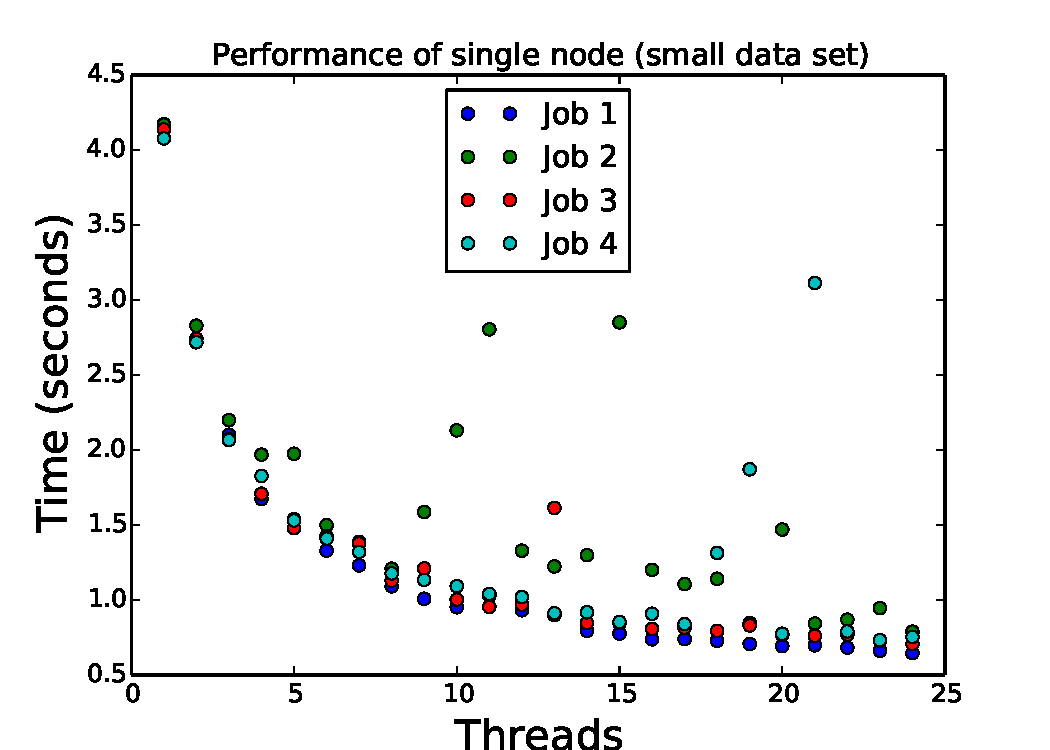
\includegraphics[width=0.8\textwidth]{SingleTime.pdf}
  \end{center}
  \caption{Absolute run-time versus threads (Small data set)} \label{fig:small_single_times}
\end{minipage}


\begin{minipage}{\linewidth}
  \captionsetup{type=figure}
  \begin{center}
  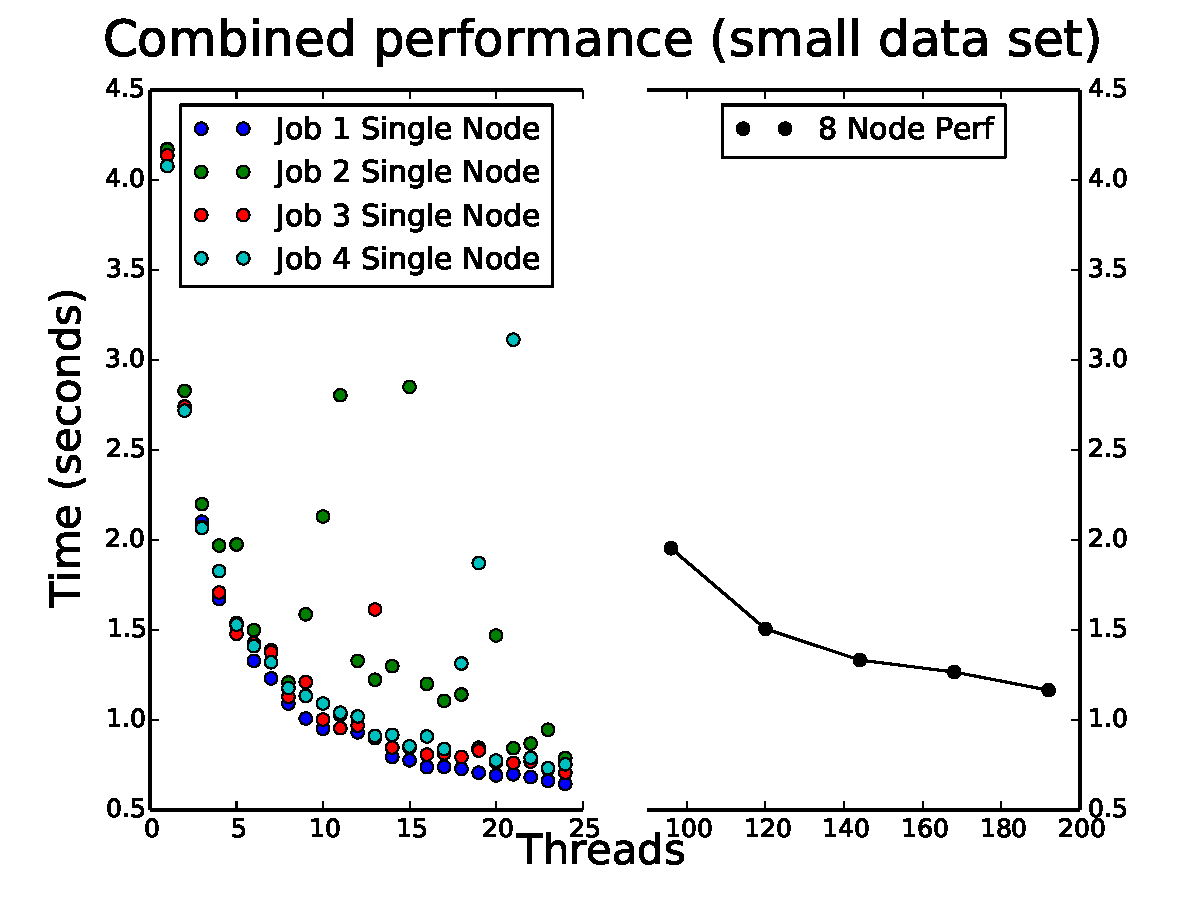
\includegraphics[width=0.8\textwidth]{CombineTimes.pdf}
  \end{center}
  \caption{Distribution of start kmers to address space (Small data set)} \label{fig:small_mult_times}
\end{minipage}

Figure~\ref{fig:small_single_times_scaling} shows how our algorithm scales on the small test verses idealized performance, as given by the formula $\frac{time_0/t}{time_t}$. The Ivy Bridge design links pairs of cores to shared memory buses. Given that our code is not cache-optimized, we expect minimal gains past 12 threads. Figure~\ref{fig:small_single_times} supports this.

\begin{minipage}{\linewidth}
  \captionsetup{type=figure}
  \begin{center}
  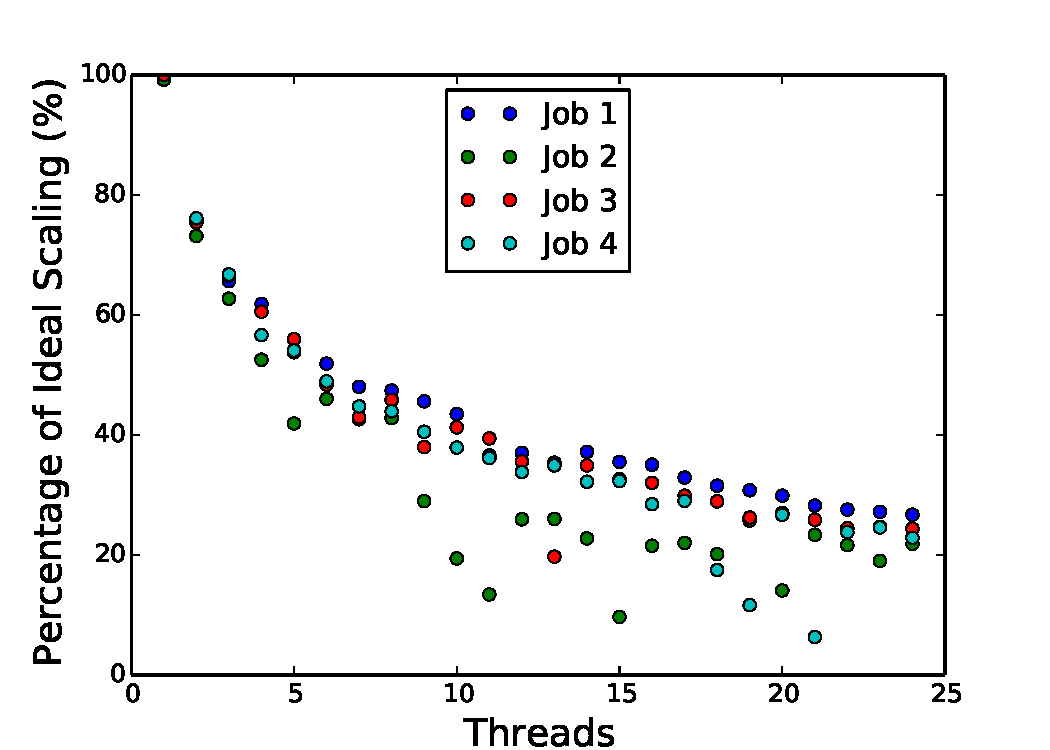
\includegraphics[width=0.8\textwidth]{SingleScaling.pdf}
  \end{center}
  \caption{Scaling versus threads (Small data set)} \label{fig:small_single_times_scaling}
\end{minipage}

Figure~\ref{fig:large_mult_times} shows absolute run-times for varying numbers of threads for the large dataset. Our algorithm took 30 seconds to perform this operation using a single thread, so we achieve a 4x speed-up for the largest numbers of threads used. However, Figure~\ref{fig:large_mult_times_scaling} shows that this represents abysmal scaling.

\begin{minipage}{\linewidth}
  \captionsetup{type=figure}
  \begin{center}
  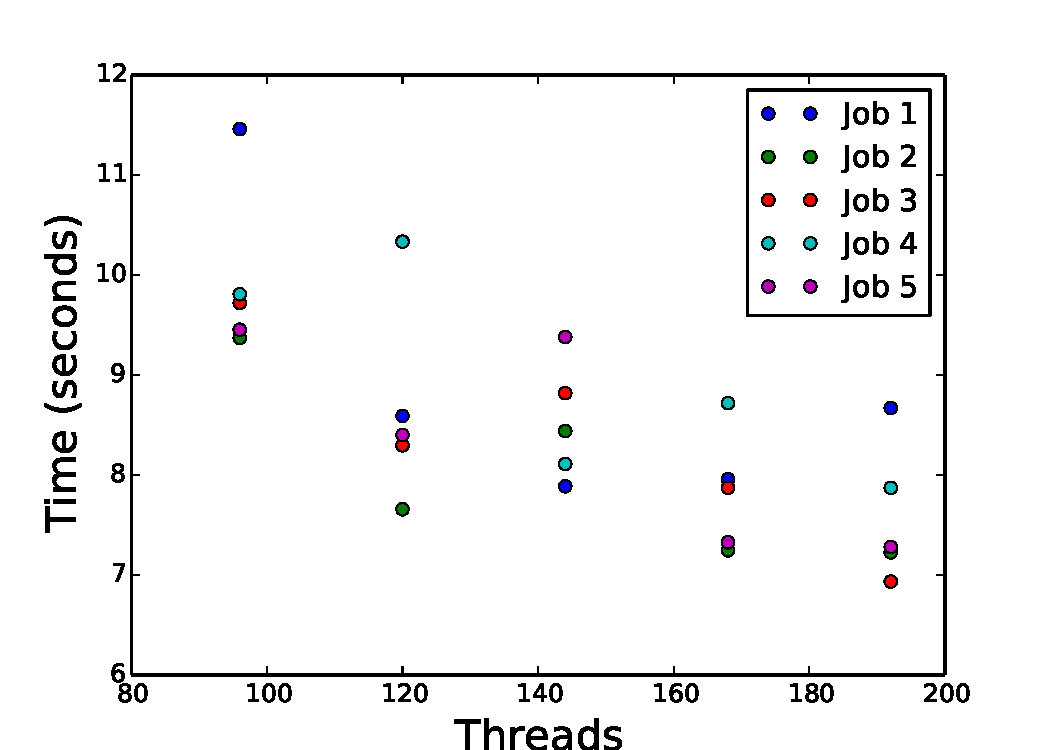
\includegraphics[width=0.8\textwidth]{LargeMultTime.pdf}
  \end{center}
  \caption{Absolute run-times versus threads (Large data set)} \label{fig:large_mult_times}
\end{minipage}


\begin{minipage}{\linewidth}
  \captionsetup{type=figure}
  \begin{center}
  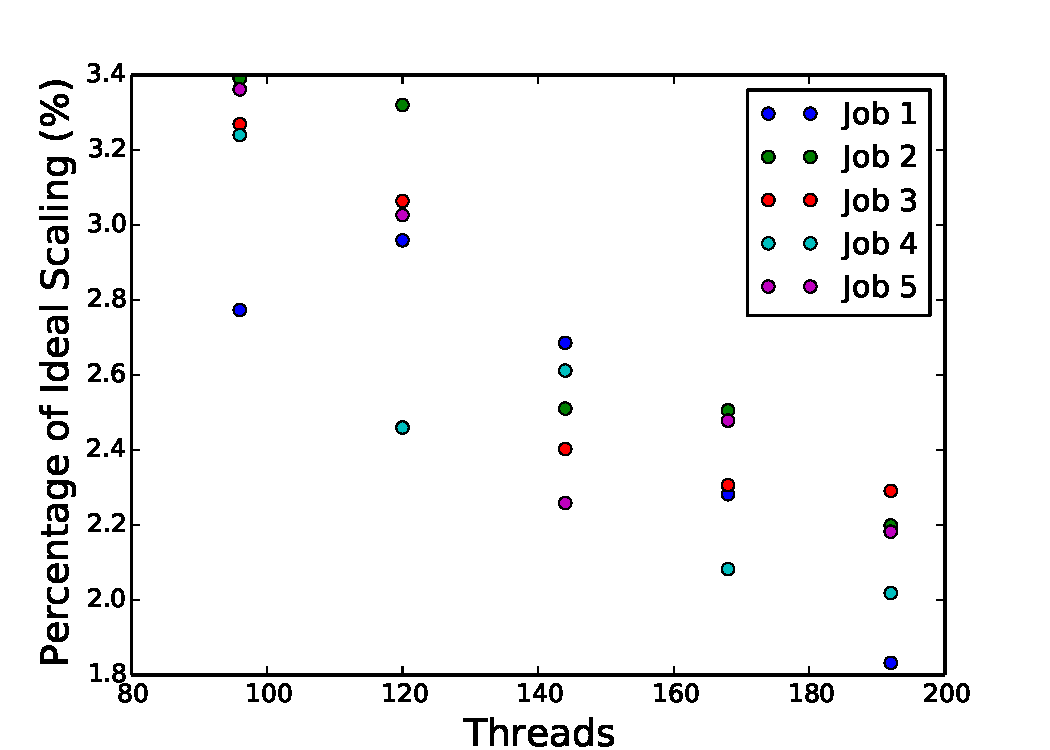
\includegraphics[width=0.8\textwidth]{LargeMultScaling.pdf}
  \end{center}
  \caption{Scaling versus threads (Large data set)} \label{fig:large_mult_times_scaling}
\end{minipage}

We hypothesized that the poor scaling was due to the high volumes of internode communication necessary to explore the hashtable. To test this, we ran the big dataset on a single node with various numbers of threads. As shown in Figure~\ref{fig:multi_single_and_big} this achieves faster performance than dividing the work between eight nodes.

\begin{minipage}{\linewidth}
  \captionsetup{type=figure}
  \begin{center}
  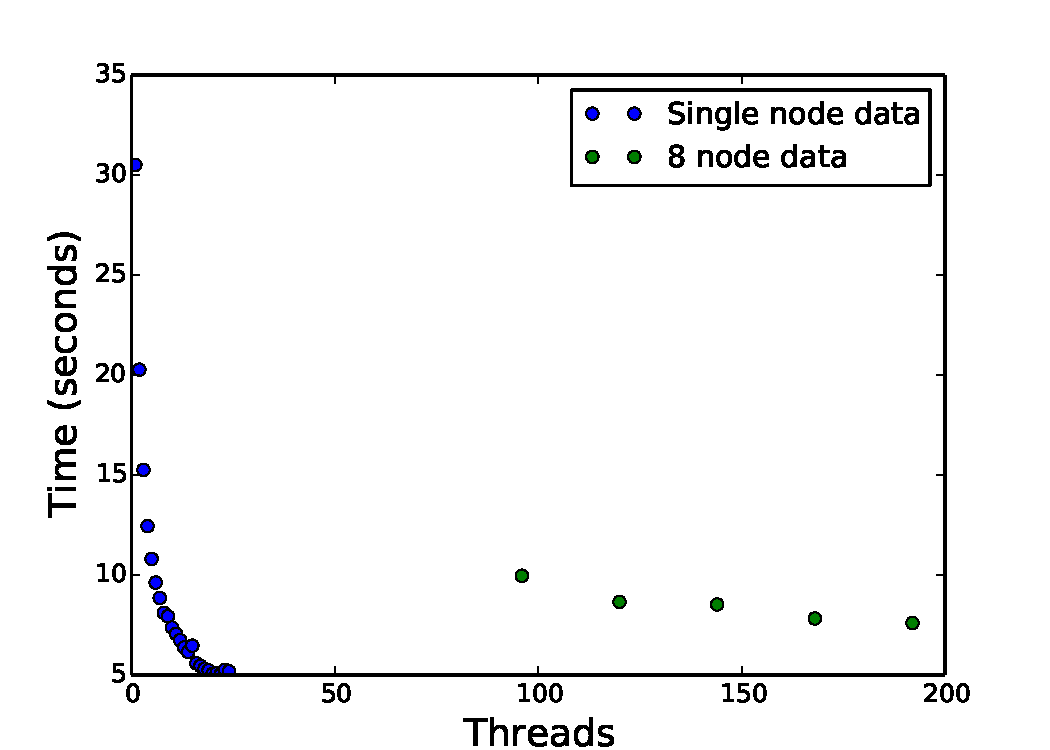
\includegraphics[width=0.8\textwidth]{MultiANDSingleBIGtime.pdf}
  \end{center}
  \caption{Absolute time versus threads including a single node (Large data set)} \label{fig:multi_single_and_big}
\end{minipage}

As Figure~\ref{fig:multi_single_and_big_scaling} shows, the run-times we see running on eight nodes seem to be part of the same scaling curve the single node experiences.

\begin{minipage}{\linewidth}
  \captionsetup{type=figure}
  \begin{center}
  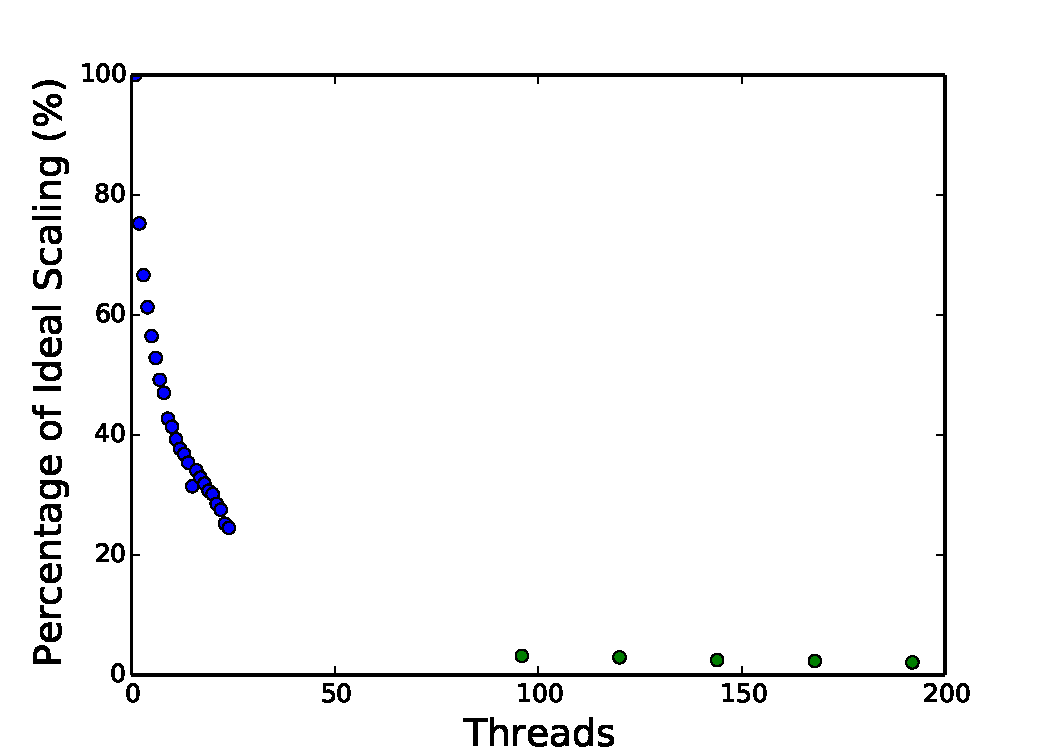
\includegraphics[width=0.8\textwidth]{MultiANDSingleBIGScaling.pdf}
  \end{center}
  \caption{Scaling versus threads including a single node (Large data set)} \label{fig:multi_single_and_big_scaling}
\end{minipage}

This suggests that the scaling is somehow inherent to the algorithm. The computational motif most strongly associated with our algorithm is ``graph traversal". The Berkeley View Dwarf Mine states that many current computer architectures fail to efficiently handle this motif because ``most searching algorithms end up depending almost entirely on random memory access latency". In our case, accessing random memory means utilizing relatively expensive communication channels (especially expensive when these channels are between nodes), so it should not be surprising that additional processing power does not translate to significantly better runtimes: many of the threads are competing for access to memory! This is true even with striped file access due to L1 and L2 caches. UPC still seems like a good choice for this motif since the computation requires large memories and every other way we've covered for distributed memory would have even higher communication costs. Perhaps further progress would be made by having exceptionally light-weight processes run on all but the first node: these processes would do no computation, but allow access to their shared memory.

Figure~\ref{fig:split} shows a break-down of the run-times of our algorithm for various numbers of threads showing the costs of both graph construction and traversal. As might be expected, construction takes longer than traversal, but the two follow similar curves. Therefore, optimizing construction is likely to bring gains regardless of communication details or other factors. 

\begin{minipage}{\linewidth}
  \captionsetup{type=figure}
  \begin{center}
  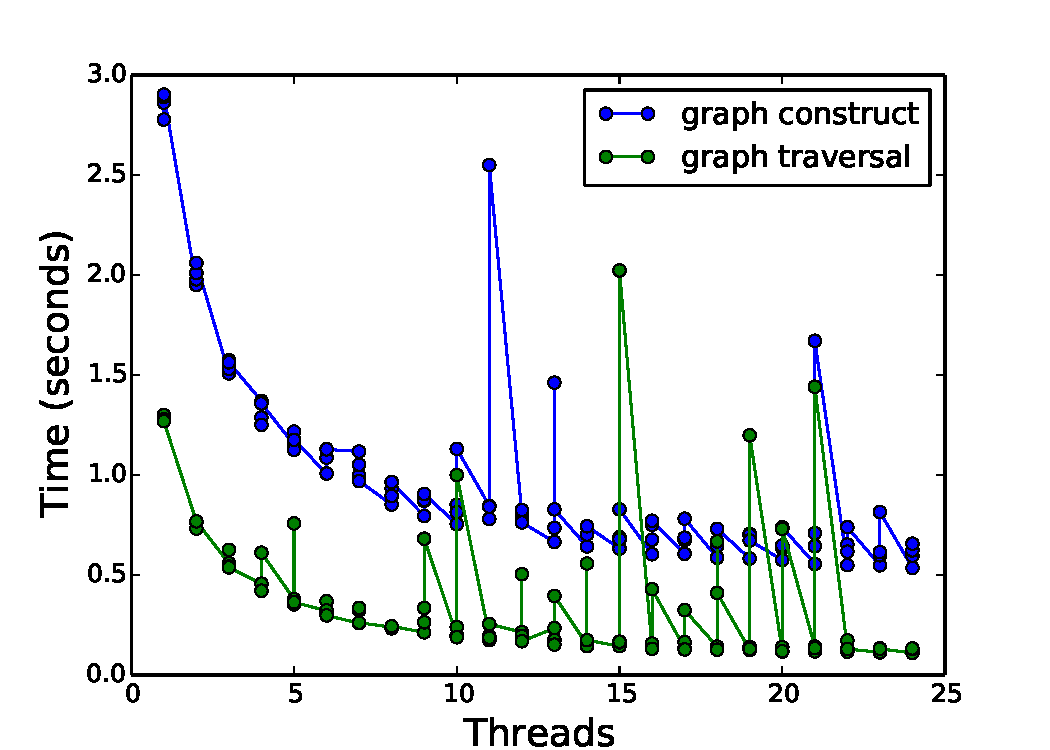
\includegraphics[width=0.8\textwidth]{single_split_time.pdf}
  \end{center}
  \caption{Absolute run-times versus threads for a single node showing break down by part of algorithm (Large data set)} \label{fig:split}
\end{minipage}

Likewise, it's possible that optimizing for our algorithm's communication motif could be helpful. Our algorithm uses round robin node-to-node communication for building the hashtable and limited scatter operations for during memory allocation. Traversal is accomplished with essentially random node-to-node communication. Thus, a fully-connected (or close to) architecture is useful for us. Given the small numbers of nodes involved, this may be technically and monetarily feasible.











\begin{comment}
Before coding up the genome assembly in parallel, we will first describe the approach for shotgun de novo genome assembly with a serial algorithm for comparison with setting up a UPC algorithm. Algorithm~\ref{serial} shows a cleaned up version of the main bulk of the code while Algorithms~\ref{packingDNAseq}--~\ref{contig_generation} show the code used to define packing routines and structures for the kmers. Overall one can see that there are three parts to the code: (1) Initialization of kmer values and hash table memory, (2) De Bruijn Graph Construction, (3) De Bruijn Graph Traversal. 

The code takes the input to be a set of unique k-mers along with their corresponding forward and backward extensions. To denote start/terminating kmer for a contig, there is a possibility of an extension being a ``guard" extension F which is incorporated into the hash table. We assume that the unique kmers have already been screened for errors so that the first step of the algorithm is to read in the unique values and construct a hash table with keys equal to the kmer and values equal to the forward and backward extensions. As shown in Algorithm~\ref{serial} the hash table is initialized with pre-allocated memory.  Within the graph construction step, the hash table is populated and a Start list is created to denote which Kmers will begin a contig. 

After the hash table has been populated, the Graph Traversal step begins by looping through the kmer Start list, which provides a ``seed" for the contigs that are created. Each traversal seed is added onto by appending the  the forward extension to the last n-1 k-mer values (where n is the kmer length defined in ~\ref{contig_generation}) and referring to the hash table for the next forward extension. This process is continued until a ``guard" extension is reached, at which point the contig is finished and printed to an external file. 

Within the serial code, many external functions and variables are referenced which were defined in Algorithms~\ref{packingDNAseq}- ~\ref{contig_generation}. These are displayed below the serial implementation code.
\end{comment}

\begin{comment}
\begin{table}
    \begin{tabular}[t]{|c|p{3.2cm}|}
        \hline
        &Alg. ~\ref{packingDNAseq} (packing sequences)\\ \hline
        1&\emph{Function} for initial lookup of kmers \\ \hline
        2&\emph{Function} to convert FourMer to packed\\ \hline
        3&\emph{Function} to pack sequences \\ \hline   
        4&\emph{Function} to unpack sequences \\ \hline
        5&\emph{Function} to compare packed sequences \\ \hline   
    \end{tabular}
    \hfill
    \begin{tabular}[t]{|c|p{3.2cm}|}
        \hline
        &Alg. ~\ref{kmer_hash} (kmer hashing)\\ \hline
        1&\emph{Function} to create hash table and pre-allocate memory\\ \hline
        2&\emph{Function} to compute hash sequence values \\ \hline
        3&\emph{Function} to return hash value of a kmer \\ \hline   
        4&\emph{Function} to look up Kmer and return a pointer to it\\ \hline
        5&\emph{Function} to add a kmer to hash table\\ \hline   
        6&\emph{Function} to add a kmer to start list  \\ \hline     
        7&\emph{Function} to deallocate memory buffers\\ \hline     
        8&\emph{Function} to deallocate hash table memory\\ \hline     
    \end{tabular}
    \hfill
    \begin{tabular}[t]{|c|p{3.2cm}|}
        \hline
        &Algorithm ~\ref{contig_generation} (contig generation) \\ \hline
        1&\emph{Function} for time keeping\\ \hline
        2&\emph{Structure} for Kmer data \\ \hline
        3&\emph{Structure} for start-kmer \\ \hline   
        4&\emph{Structure} for buckets\\ \hline
        5&\emph{Structure} for hash table \\ \hline   
        6&\emph{Structure} for working memory buffers\\ \hline   
        7&\emph{Function} for getting number of Kmers in file \\ \hline   
    \end{tabular}
    \caption{Functions and Structures included in Algotithms~\ref{packingDNAseq}- ~\ref{contig_generation}}
\end{table}
\end{comment}

%\mycode{serial}{Serial Implementation (C)}{code-serial.c}{c} 

%\mycode{packingDNAseq}{DNA packing routine (Fortran)}{code-packingDNAseq.h}{fortran}

%\mycode{kmer_hash}{k-mer hash table routine (Fortran)}{code-kmer_hash.h}{fortran}

%\mycode{contig_generation}{Generation of contigs routine (Fortran)}{code-contig_generation.h}{fortran}


\begin{comment}
\section{UPC approach}
The first thing to be done in the extension to UPC was to rewrite the packing and hashing functions for a PGAS framework. This gives us an initial list of start kmers ({\color{red}Elaborate on changes for these functions}). 

Next a function was built for finding the next kmer, so that graph traversal can occur in the partition global address space. This allows one to get to the point of allowing contigs to be generated({\color{red}Elaborate on changes for this function}).

At this point a choice needed to be made for the communication of PGAS threads. We decided to read input into a circular buffer that all the threads could then have blocks of dedicated address space in. ({\color{red}insert better explanation of how this buffer works?})

Later we considered the option of enabling parallel read-in capabilties, since at this point the UPC code did a sequential read in and then distributed the input accross the partitioned global memory space. This means that the only benefit from using PGAS came from having access to a large memory space, but no improvements in speed could be gained yet. 

 To perform a parallel read-in, we hoped to involve atomics on the hash table - and we consider the use of conditional swap as a method for implementing this. However, atomic procedures are not traditionally used for individual bytes and we were not able to find a Berkeley UPC atomics library. We therefore considered using UPC locks instead - which has it's own difficulties due to the inability to lock an openly addressed hash table. As an alternative strategy we decided to partition the table into blocks of 100 do locking on the individual blocks. ({\color{red}Insert code to describe how this works}) 

 This methodology works only if the probability of a lock collision is relatively small. ({\color{red}Insert part about the relative probability of collisions existing for certain hash tables... ?}) 

%stuff about number of collisions existing for different types of hash tables (amount of randomness)?
%sequence starting kmers are distributed fairly evenly throughout the test file
%more stuff about randomness of kmers being distributed being important for load balancing? In real life it is possible to randomize the line order of the file...but this means each processor can keep track of its starting-mers locally

After testing the code further at this point, numerous deadlocks were witnessed. To address this issue, we decided to try synchronized rotating access to chunks of the table - which resulted in an intiial code that was faster than the serial version. ({\color{red}Insert a figure comparing initial performance against serial version?})

In the later stages of the code, local representations of the hash tables were created to avoid synchornization issues. We also began to wonder if things could be  made faster with linked lists, which would have $\circ (1)$ insertion time and $\circ(BinN)$ retrieval time, as opposed to open hash table approaches which have $\circ (BinN)$ for both. If the circular buffer method was still applied to linked lists, then the approach could remain lock free. 

\end{comment}


\begin{comment}
figures/plots that could exist:
\begin{itemize}
\item timing plots?
\end{itemize}

List of suggested things to include from homework statement:
\begin{itemize}
\item A description of the computational and communication motifs of the parallel algorithms.
\item Discussion of the scalability and relative costs of the parallel graph construction and traversal algorithms.
\item A discussion on using UPC for such an application with the underlying computational motif.
\end{itemize}

\section{Performance}
\begin{itemize}
\item Simple compared results against serial implementation.
\end{itemize}

\section{Summary}
\end{comment}


\end{document}
